% !TeX root = main.tex
\chapter{Theoretical Background}

Topics to consider when starting the Sensor Health Monitoring process are mainly that of providing a structured
overview of the Sensor Metadata which in itself consists of many layers as a dynamically generated set of metadata is
desired. This should be able to accomodate changing Data Acquisitioning (DAQ) System configuration changes.
Consideration is given to the SOIL data model and its' ability to accomodate the many demands that are expected of
sensor data management. \cite{SOIL model}
The second major part to consider is that of physical crossrelations and \"deep checks\" which are a experimental mode of checking for inconsistencies among the data.
Major research and implementation work shall go into developing a dynamic model that is generated from the data and then checks back upon the data for possible discrepancies. This approach is chosen as it is estimated to be the most structured approach for a first prototype.



\begin{figure}[h]
         \centering
         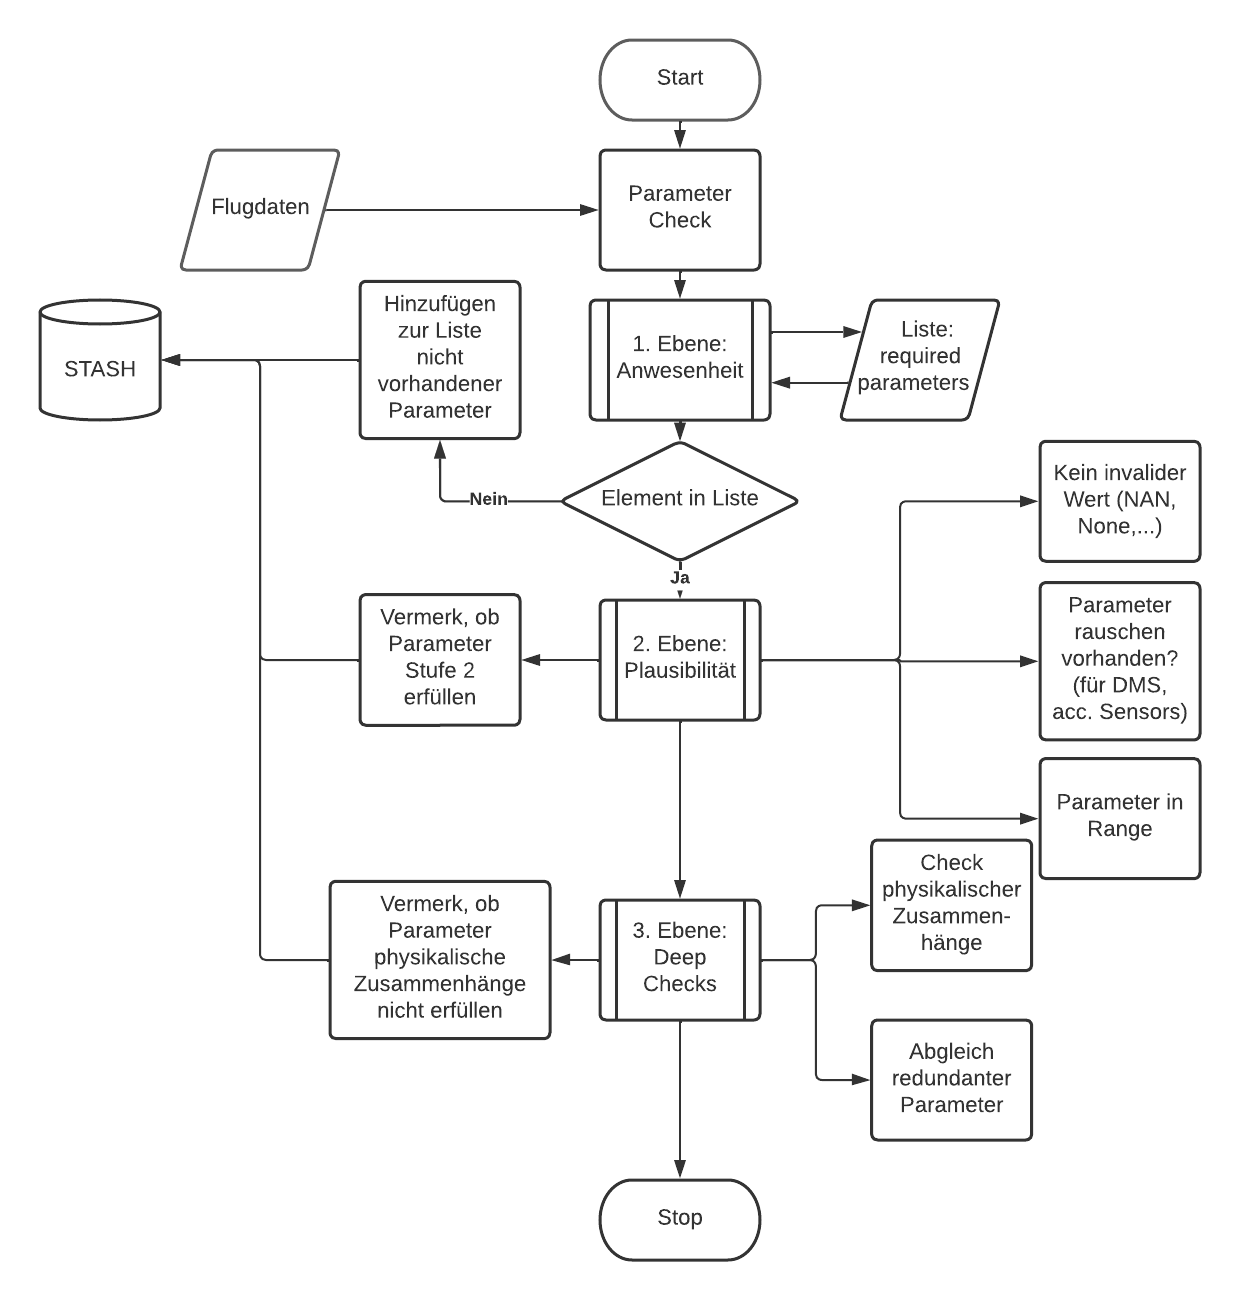
\includegraphics[width=1\textwidth]{SensorHealthMonitoring}
         \caption{}
         \label{fig:}
\end{figure}

\section{control systems approach}

Following the recipe for a modeled aircraft based on sensor data we try to simulate the parameters x and u of the
aircraft with the sensor data y. Khaled shows that this approach works for linking omega_x omega_y, delta_delta
(drift angle) with
omega_z.


To achieve rigorousness... \cite[80]{HEVN04}

\cite{HEVN04}


\Blindtext[10]

\section{test-section}

\Blindtext[4]